\section{Les systèmes de télécommunications sans fil}
Si la dénomination de « \textbf{systèmes de télécommunications} »
(\textit{telecommunication systems}) paraît quelque peu abstraite, elle englobe
en réalité un grand nombre d'objets et équipements qui nous sont très familiers.
This first part fixes what such a system is, what all of them have in common,
why they are operated at radio frequencies rather than at the audio frequencies
of a first electronics course, and what makes radio-frequency engineering a
different discipline from electronics at basse fréquence. It ends on the single
problem that organises the whole module: a signal radiofréquence loses power
everywhere it goes, and the two engineering answers to that are amplification
and adaptation d'impédance.

\subsection{Systèmes de télécommunications}

\begin{definition}[Système de télécommunications]
  Les \textbf{systèmes de télécommunications} émettent et reçoivent de
  l'information (voix, vidéo, fichiers, données en streaming) grâce à des
  ondes électromagnétiques qui sont rayonnées et captées par des antennes. Ils
  contiennent des circuits électroniques émetteurs et récepteurs.
\end{definition}

The course splits the field by market volume rather than by physics, because the
volume drives the engineering constraints.

\paragraph{Applications grand public} Les systèmes de télécommunications sont
pour la plupart des objets que nous utilisons au quotidien : smartphones,
tablettes, boxes internet, systèmes de navigation GPS (\textit{Global
Positioning System}), oreillettes Bluetooth, montres connectées, radars d'aide à
la conduite automobile, antenne parabolique et \textbf{démodulateur}
(\textit{demodulator}) pour réception de TV par satellite. Tous ces appareils
sont utilisés dans des \textbf{applications grand public} (\textit{consumer
applications}) : volume de ventes très important, chiffrés en millions ou
milliards d'unités.

\paragraph{Applications spécialisées} En plus des applications grand public, il
existe également des systèmes de télécommunications dédiés à des applications
dites spécialisées (volume de ventes très modeste, chiffré en centaines voire
dizaines d'unités). Il s'agit des satellites en orbite autour de la Terre, qui
permettent les prévisions météorologiques, la réception de TV par satellite, la
radioastronomie, l'observation de l'évolution de la déforestation ou la fonte
des glaces. Un autre type d'application spécialisée concerne les activités
militaires et de défense : radars de détection et surveillance, systèmes
d'armement, de \textbf{brouillage} (\textit{jamming}), de guidage de missiles,
communications militaires sécurisées.

\begin{remark}
  Les antennes utilisées dans ces applications se différencient par leur forme,
  leur taille, leurs performances et caractéristiques techniques. There is no
  universal antenne: il existe toutes sortes d'antennes répondant chacune à des
  contraintes particulières en fonction des applications visées. The module
  later surveys antennes filaires, antennes à ouverture rayonnante, antennes à
  réflecteur, antennes planaires and antennes réseaux for exactly that reason.
\end{remark}

\subsection{Quelles sont les caractéristiques des systèmes de télécommunications ?}
Comme nous venons de le voir, les systèmes de télécommunications sont utilisés
dans des applications très différentes et cependant, ils possèdent 3 points
communs.

\paragraph{1. Ils rayonnent et captent des ondes électromagnétiques}
Les systèmes de télécommunications émettent et reçoivent de l'information grâce
à des \textbf{ondes électromagnétiques} (\textit{electromagnetic wave}, OEM) qui
sont rayonnées en \textbf{émission}
(\textit{transmission}) et captées en réception par des antennes.
In the canonical picture --- une communication entre un smartphone émettant une
onde électromagnétique et une \textbf{station de base} (\textit{base station},
BTS, \textit{Base Transceiver Station}) recevant cette onde --- les champs
électrique $E$ et magnétique $H$ sont orthogonaux entre eux et orthogonaux à
la direction de propagation (définie par le vecteur d'onde) de l'onde.

\begin{definition}[Longueur d'onde]
  La \textbf{longueur d'onde} (\textit{wavelength}) $\lambda$ est la fréquence
  spatiale de l'onde électromagnétique. Avec $f$ la fréquence du signal et $c$
  la vitesse de la lumière,
  \[\lambda=\frac{c}{f},\qquad c \simeq 3\times 10^{8}\ \text{m/s}.\]
\end{definition}

Propagation libre ou guidée d'une onde électromagnétique : \textit{libre} in
\textbf{espace libre} (\textit{free space}), \textit{guidée} in a ligne de
transmission or a cable, which is \textbf{propagation guidée} (\textit{guided propagation}). Both
cases are governed by the same équations de Maxwell. Un rappel des notions de
base en électromagnétisme sera fait dans la deuxième partie.

\paragraph{2. Les ondes sont des signaux radiofréquence}
\begin{definition}[Signal radiofréquence]
  Les ondes électromagnétiques utilisées par les systèmes de télécommunications
  sont des \textbf{signaux radiofréquence} (\textit{radio-frequency signal},
  RF), c'est-à-dire des signaux dont
  la fréquence est approximativement comprise entre $100$ MHz et $100$ GHz.
\end{definition}

Ces fréquences sont donc très élevées… en tout cas bien plus élevées que les
fréquences que vous avez utilisées en cours d'électronique
($1$ kHz\,--\,$100$ kHz) jusqu'à présent. La figure ci-dessous présente les
bandes de fréquences RF utilisées par les systèmes de télécommunications : c'est
le \textbf{spectre radiofréquence} (\textit{radio-frequency spectrum}).

\begin{figure}[h!]
  \centering
  \begin{tikzpicture}[font=\tiny,>=stealth,
      band/.style={draw,fill=black!6,align=center,inner sep=1.5pt,rounded corners=1pt},
      ovl/.style={draw,fill=black!12,align=center,inner sep=1.5pt,rounded corners=1pt}]
    % axis
    \draw[->,thick] (0,0) -- (13.4,0) node[below right,font=\scriptsize] {fréquence (GHz)};
    \foreach \x in {0.9,2.3,3.5,4.5,5.4,6.8,8.6,10.1,12.0}
      \draw[thick] (\x,-0.09) -- (\x,0.09);
    % spectrum breaks
    \foreach \x in {9.4,10.75}
      {\draw (\x-0.07,-0.16) -- (\x+0.07,0.16); \draw (\x+0.06,-0.16) -- (\x+0.2,0.16);}
    % tick labels
    \node[below] at (0.9,-0.12) {$0{,}7-1$};
    \node[below] at (2.3,-0.12) {$1{,}575$};
    \node[below] at (3.5,-0.12) {$1{,}7-2{,}2$};
    \node[below] at (4.5,-0.12) {$2{,}4$};
    \node[below] at (5.4,-0.12) {$2{,}5-2{,}7$};
    \node[below] at (6.8,-0.12) {$3{,}4-3{,}8$};
    \node[below] at (8.6,-0.12) {$5{,}1-5{,}9$};
    \node[below] at (10.1,-0.12) {$24$};
    \node[below] at (12.0,-0.12) {$76-81$};
    % first row of service boxes
    \node[band,minimum width=1.2cm] (a) at (0.9,0.85) {GSM, EDGE\\HSPA, LTE-A};
    \node[band,minimum width=1.2cm] (b) at (3.5,0.85) {GSM, EDGE\\HSPA, LTE-A};
    \node[band,minimum width=1.0cm] (c) at (5.4,0.85) {HSPA, LTE\\LTE-A};
    \node[band,minimum width=0.9cm] (d) at (6.8,0.85) {5G};
    \node[band,minimum width=1.0cm] (e) at (8.6,0.85) {Wi-Fi};
    \node[band,minimum width=1.4cm] (f) at (12.0,0.85) {Radars\\automobiles};
    \foreach \n in {a,b,c,d,e,f} \draw (\n.south) -- ($(\n.south)+(0,-0.42)$);
    % second row
    \node[band,minimum width=1.0cm] (g) at (2.3,2.05) {GPS\\Galileo};
    \node[band,minimum width=1.2cm] (h) at (4.5,2.05) {Wi-Fi\\Bluetooth\\ZigBee};
    \node[band,minimum width=1.4cm] (i) at (10.1,2.05) {Radars\\automobiles};
    \foreach \n in {g,h,i} \draw[->] (\n.south) -- ($(\n.south)+(0,-1.62)$);
    % overlay service bars
    \draw[ovl] (2.3,2.95) rectangle (10.75,3.35);
    \node at (6.5,3.15) {Aerospace \& Satellite (1--40 GHz, discontinuous)};
    \node[right,font=\tiny] at (10.85,3.15) {40 GHz};
    \draw[ovl] (2.3,3.55) rectangle (13.1,3.95);
    \node at (7.7,3.75) {Military \& Defence (1--100 GHz, discontinuous)};
    \node[right,font=\tiny] at (13.2,3.75) {100 GHz};
  \end{tikzpicture}
  \caption*{\small Spectre radiofréquence (RF) \& applications. The most common
  consumer services all sit below $6$ GHz; satellite ($1$--$40$ GHz) and defence
  ($1$--$100$ GHz) overlay much of the spectrum, including part of the sub-$6$ GHz
  range, and use it discontinuously.}
\end{figure}

Les fréquences allouées aux applications les plus couramment utilisées
(téléphonie mobile, Wi-Fi, GPS, Bluetooth) sont situées à des fréquences
inférieures à $6$ GHz. Les satellites opèrent globalement entre $1$ GHz et
$40$ GHz mais avec une utilisation du spectre de manière \textit{discontinue} :
un satellite A utilise la bande de fréquences entre $1$\,--\,$2$ GHz, un
satellite B entre $4$\,--\,$6$ GHz, un satellite C entre $8$\,--\,$12$ GHz… et
certaines bandes de fréquences ne sont pas utilisées. Quant aux applications
militaires \& défense, elles sont présentes entre $1$\,--\,$100$ GHz de manière
également discontinue.

\begin{conclusion}
  La quasi-totalité des fréquences du spectre RF sont dédiées à une ou
  plusieurs applications : le spectre RF est \textit{saturé}. Spectrum is a
  scarce resource, which is why band allocations are fought over and why
  services are retired to free them. The GSM and EDGE allocations at
  $0{,}7$\,--\,$1$ GHz and $1{,}7$\,--\,$2{,}2$ GHz are scheduled for shutdown by
  the end of $2028$.
\end{conclusion}

\begin{remark}
  The upper automotive-radar band is quoted either as $76$\,--\,$79$ GHz or as
  $76$\,--\,$81$ GHz; the figure above uses the wider range. Either way the band
  sits in the millimetre-wave region just below $100$ GHz.
\end{remark}

\paragraph{3. Ils contiennent des circuits émetteurs et récepteurs}
Les systèmes de télécommunications contiennent des circuits électroniques
\textbf{émetteurs} (\textit{transmitters}, Tx) et \textbf{récepteurs}
(\textit{receivers}, Rx). Si les antennes constituent la partie visible de ces
émetteurs/récepteurs (même si les antennes sont de plus en plus cachées), elles
rayonnent et captent des signaux RF qui sont générés, modulés/démodulés,
mélangés, amplifiés, filtrés par des circuits électroniques qui eux, sont
toujours cachés.

\subsection{La propagation dans les systèmes de télécommunication numérique}
A modern system is digital at both ends and analogue in the middle. Supposons
que les bits de données $01101110\ldots$ --- voice, video, data --- doivent être
transmis au récepteur.

\begin{figure}[h!]
  \centering
  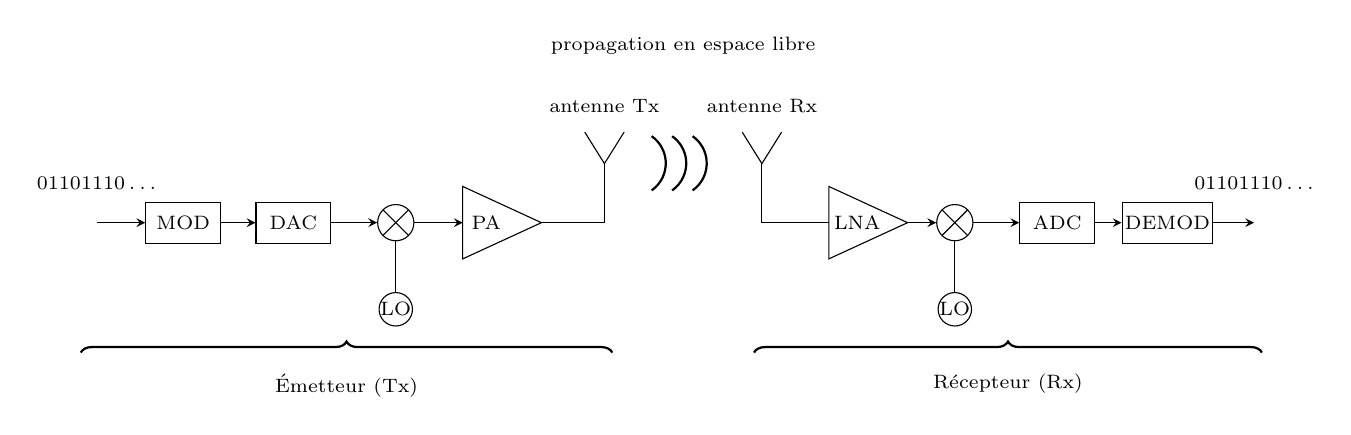
\begin{tikzpicture}[font=\scriptsize,>=stealth,
      blk/.style={draw,minimum width=0.95cm,minimum height=0.52cm,inner sep=1pt}]
    % --- transmitter ---
    \node[blk] (mod) at (0.6,0) {MOD};
    \node[blk] (dac) at (2.0,0) {DAC};
    \node[draw,circle,minimum size=0.46cm,inner sep=0pt] (mx1) at (3.3,0) {};
    \draw (mx1) ++(-0.16,-0.16) -- ++(0.32,0.32); \draw (mx1) ++(-0.16,0.16) -- ++(0.32,-0.32);
    \draw (4.15,-0.46) -- (4.15,0.46) -- (5.15,0) -- cycle;
    \node at (4.45,0) {PA};
    \node[draw,circle,minimum size=0.42cm,inner sep=0pt] (lo1) at (3.3,-1.1) {LO};
    \draw (mx1) -- (lo1);
    \draw[->] (-0.5,0) -- (mod.west);
    \node[align=center] at (-0.5,0.5) {$01101110\ldots$};
    \draw[->] (mod) -- (dac); \draw[->] (dac) -- (mx1);
    \draw[->] (mx1) -- (4.15,0);
    % Tx antenna
    \draw (5.15,0) -- (5.95,0) -- (5.95,0.75);
    \draw (5.70,1.15) -- (5.95,0.75) -- (6.20,1.15);
    \node[align=center] at (5.95,1.48) {antenne Tx};
    % --- propagation ---
    \foreach \i in {0,1,2} \draw[thick] (6.55+0.26*\i,0.41) arc (-55:55:0.42);
    \node[align=center] at (6.95,2.25) {propagation en espace libre};
    % --- receiver ---
    \draw (7.95,0.75) -- (7.95,0) -- (8.80,0);
    \draw (7.70,1.15) -- (7.95,0.75) -- (8.20,1.15);
    \node[align=center] at (7.95,1.48) {antenne Rx};
    \draw (8.80,-0.46) -- (8.80,0.46) -- (9.80,0) -- cycle;
    \node at (9.16,0) {LNA};
    \node[draw,circle,minimum size=0.46cm,inner sep=0pt] (mx2) at (10.4,0) {};
    \draw (mx2) ++(-0.16,-0.16) -- ++(0.32,0.32); \draw (mx2) ++(-0.16,0.16) -- ++(0.32,-0.32);
    \node[draw,circle,minimum size=0.42cm,inner sep=0pt] (lo2) at (10.4,-1.1) {LO};
    \draw (mx2) -- (lo2);
    \node[blk] (adc) at (11.7,0) {ADC};
    \node[blk] (dem) at (13.1,0) {DEMOD};
    \draw[->] (9.80,0) -- (mx2); \draw[->] (mx2) -- (adc); \draw[->] (adc) -- (dem);
    \draw[->] (dem.east) -- (14.2,0);
    \node[align=center] at (14.2,0.5) {$01101110\ldots$};
    % brace labels
    \draw[decorate,decoration={brace,amplitude=4pt},thick] (-0.7,-1.65) -- (6.05,-1.65)
      node[midway,below=4pt] {Émetteur (Tx)};
    \draw[decorate,decoration={brace,amplitude=4pt},thick] (7.85,-1.65) -- (14.3,-1.65)
      node[midway,below=4pt] {Récepteur (Rx)};
  \end{tikzpicture}
  \caption*{\small Schéma fonctionnel simplifié d'une communication RF.
  Everything between the DAC and the ADC is analogue.}
\end{figure}

Au niveau de l'émetteur, les bits sont soumis à un traitement numérique appelé
\textbf{modulation} (MOD) suivi d'une \textbf{conversion numérique/analogique}
(\textit{digital-to-analogue conversion}, DAC). Celle-ci consiste en la
conversion des bits de données (numérique) en signal analogique
\textbf{basse fréquence} (\textit{low frequency}, BF). À la sortie
du DAC, un \textbf{mélangeur} (\textit{mixer}) permet la transposition de ce
signal analogique BF vers les fréquences RF. Le terme « mélangeur » provient du
fait que le signal basse fréquence sortant du DAC est « mélangé » à un signal
haute fréquence provenant d'un \textbf{oscillateur local} (\textit{local
oscillator}, LO) pour donner un signal RF en sortie du mélangeur. Un
\textbf{amplificateur de puissance} (\textit{power amplifier}, PA) augmente alors
la puissance de ce signal RF qui est ensuite rayonné par l'antenne d'émission
(Tx).\\

Après s'être propagé dans l'air (subissant un très fort affaiblissement), le
signal RF est capté par l'antenne de réception (Rx). Le signal RF étant très
faible, un \textbf{amplificateur faible bruit} (\textit{low-noise amplifier},
LNA) est alors utilisé pour élever le niveau du signal reçu, puis un mélangeur
transpose le signal RF vers les fréquences BF. Enfin, un \textbf{convertisseur
analogique/numérique} (\textit{analogue-to-digital converter}, ADC) transforme
le signal analogique BF sous forme numérique, puis celui-ci est démodulé
(DEMOD) et les bits de données $01101110\ldots$ sont récupérés.

\begin{conclusion}
  En pratique, ce schéma peut illustrer la communication entre un smartphone et
  sa station de base, entre une box internet et le module Wi-Fi d'un PC, entre
  un smartphone et une enceinte Bluetooth, entre un satellite GPS et le module
  GPS installé dans une voiture. Whatever the service, the chain is the same,
  and the quantity that actually propagates is a \textbf{signal sinusoïdal
  analogique}. This is why a module on propagation and antennes is stated
  entirely in terms of sinusoidal waves even though the traffic is digital.
\end{conclusion}

\begin{example}[Digital modulation schemes]
  The digital modulator maps bits onto the parameters of a sinusoid:
  \begin{subpart}
    \item \textbf{Modulation d'amplitude} (\textit{amplitude modulation}), e.g.\
      OOK (\textit{on-off keying}):
      a burst of carrier means $1$, no carrier means $0$. The frame
      $10100110$ appears as bursts separated by silences.
    \item \textbf{Modulation de fréquence} (\textit{frequency modulation}),
      e.g.\ FSK (\textit{frequency-shift
      keying}): each symbol selects one of several carrier frequencies; with
      four tones a symbol carries two bits, $00$, $01$, $10$, $11$. The frame
      $10110100$ splits into the symbols $10$, $11$, $01$, $00$; the tone
      assignment runs fastest-to-slowest as $11$, $10$, $01$, $00$, so the $11$
      burst is the densest and the $00$ burst the sparsest.
    \item \textbf{Modulation de phase} (\textit{phase modulation}), e.g.\ BPSK
      (\textit{binary phase-shift
      keying}): $1$ and $0$ are carried by two carrier phases $\pi$ apart. The
      frame $10011010$ appears as a continuous sinusoid with phase reversals at
      the symbol boundaries.
  \end{subpart}
\end{example}

\subsection{Quel est l'intérêt de faire fonctionner ces systèmes aux fréquences RF ?}
Les fréquences RF sont utilisées dans les systèmes de communications pour
3 raisons principales.

\paragraph{1. La taille des antennes varie en $1/f$}
La taille des antennes varie de manière inversement proportionnelle à la
fréquence. Les antennes sont donc plus petites aux fréquences RF et sont ainsi
plus facilement intégrables dans des boîtiers au milieu de différents circuits
électroniques. The progression from an antenne cornet large enough to fill a
laboratory bench at $0.1$ GHz down to the few-millimetre antenne hidden inside
a mobile phone at $100$ GHz is a direct consequence of $\lambda=c/f$.

\paragraph{2. Les conditions de propagation sont relativement favorables}
Les signaux RF se propagent convenablement en milieu urbain, ils sont capables
de traverser les murs des bâtiments, les vitres, les parois des véhicules, la
végétation, ils sont relativement insensibles aux conditions climatiques ---
wind, rain, snow.

\begin{remark}
  Il convient cependant de rester mesuré lorsque l'on parle de conditions de
  propagation favorables pour les signaux RF. En effet, les ondes
  électromagnétiques se propagent avec une atténuation d'autant plus forte que
  la fréquence est élevée… et les fréquences RF étant par définition des
  fréquences très élevées, elles subissent par conséquent une très forte
  atténuation… qui peut cependant être compensée par amplification des signaux
  et adaptation d'impédance --- the subject of the rest of this part. Note
  also, with feeling, that the window glass of Télécom Paris is the exception
  that does not let RF through.
\end{remark}

\paragraph{3. Les larges bandes spectrales sont disponibles}
La transmission de données haut débit nécessite l'utilisation d'une large
bande de fréquence. Un signal qui transporte de l'information est un
\textbf{signal modulé} (\textit{modulated signal}) et un tel signal occupe dans
le spectre RF une largeur de bande non nulle. De manière générale, plus un
signal occupe une bande de fréquence large, plus il favorise la transmission de
données haut débit.

\begin{figure}[h!]
  \centering
  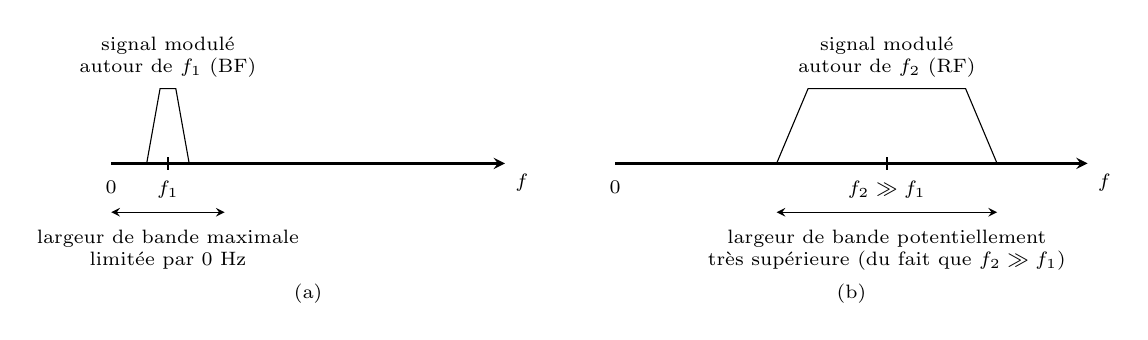
\begin{tikzpicture}[font=\scriptsize,>=stealth]
    % panel a
    \draw[->,thick] (0,0) -- (5.0,0) node[below right] {$f$};
    \draw (0.45,0) -- (0.62,0.95) -- (0.82,0.95) -- (0.99,0) -- cycle;
    \draw[thick] (0.72,-0.08) -- (0.72,0.08);
    \node[below] at (0.72,-0.1) {$f_1$};
    \node[below] at (0,-0.1) {$0$};
    \node[align=center] at (0.72,1.35) {signal modulé\\autour de $f_1$ (BF)};
    \draw[<->] (0,-0.62) -- (1.44,-0.62);
    \node[align=center,below] at (0.72,-0.72) {largeur de bande maximale\\limitée par $0$ Hz};
    \node at (2.5,-1.65) {(a)};
    % panel b
    \begin{scope}[xshift=6.4cm]
      \draw[->,thick] (0,0) -- (6.0,0) node[below right] {$f$};
      \draw (2.05,0) -- (2.45,0.95) -- (4.45,0.95) -- (4.85,0) -- cycle;
      \draw[thick] (3.45,-0.08) -- (3.45,0.08);
      \node[below] at (3.45,-0.1) {$f_2 \gg f_1$};
      \node[below] at (0,-0.1) {$0$};
      \node[align=center] at (3.45,1.35) {signal modulé\\autour de $f_2$ (RF)};
      \draw[<->] (2.05,-0.62) -- (4.85,-0.62);
      \node[align=center,below] at (3.45,-0.72) {largeur de bande potentiellement\\très supérieure (du fait que $f_2\gg f_1$)};
      \node at (3.0,-1.65) {(b)};
    \end{scope}
  \end{tikzpicture}
  \caption*{\small Signal modulé (a) autour d'une fréquence BF $f_1$ et (b)
  autour d'une fréquence RF $f_2 \gg f_1$. L'axe des abscisses représente la
  fréquence (en GHz) et l'axe des ordonnées représente la puissance du signal
  (en W).}
\end{figure}

Si on considère le cas d'un signal modulé centré sur une fréquence BF $f_1$ peu
élevée (quelques kHz ou MHz), la largeur de bande maximale de ce signal est
limitée par la fréquence $0$ Hz (car physiquement, les fréquences négatives
n'existent pas). Si on considère maintenant un signal modulé centré sur une
fréquence $f_2 \gg f_1$ située dans le spectre RF ($0.1$\,--\,$100$ GHz), sa
largeur de bande peut potentiellement être très supérieure du fait que cette
fréquence est très « éloignée » de la fréquence $0$ Hz. Only the RF-centred
signal supports high-rate data transmission.

\subsection{Spécificités de l'ingénierie RF}
Un signal RF de fréquence $1$ GHz n'est pas qu'un signal qui varie dans le
temps $10^{6}$ fois plus vite qu'un signal BF de fréquence $1$ kHz. Cela
implique aussi et surtout des effets remarquables. Les circuits RF possèdent des
spécificités qui leur sont propres et les différencient des circuits BF.

\subsubsection{L'approximation basses fréquences n'est plus valable}
L'ingénierie de l'électronique BF (montages à amplificateurs opérationnels,
amplificateur collecteur/émetteur commun, filtres actifs…) est basée sur
l'approximation qui n'est valable uniquement qu'aux fréquences BF, pour
lesquelles la longueur d'onde $\lambda=c/f$ est extrêmement grande --- that is,
large compared with the circuit. Aux fréquences RF, la longueur d'onde est petite.

\begin{figure}[h!]
  \centering
  \small
  \begin{tabular}{lccccccc}
    \toprule
    $f$       & $1$ kHz & $20$ kHz & $1$ GHz & $5$ GHz & $10$ GHz & $40$ GHz & $100$ GHz \\
    \midrule
    $\lambda$ & $30$ km & $15$ km  & $30$ cm & $6$ cm  & $3$ cm   & $7{,}5$ mm & $3$ mm \\
    \bottomrule
  \end{tabular}
  \caption*{\small $\lambda=c/f$ across the BF and RF ranges. BF circuits have
  $\lambda \approx$ km; RF circuits have $\lambda \approx$ mm to m.}
\end{figure}

Par conséquent, la taille des composants électroniques (transistors,
résistances, capacités, inductances), la longueur des pistes sur les circuits
imprimés (et circuits intégrés), et la longueur des câbles deviennent alors non
négligeables par rapport à $\lambda$ et/ou supérieures à $\lambda$.

\begin{conclusion}
  La \textbf{théorie dite des lignes de transmission} s'applique alors aux
  pistes, aux câbles et plus généralement aux circuits RF. This is the subject
  of the third part of the module.
\end{conclusion}

\begin{example}[Circuit dimensions are fractions of a wavelength]
  A $20$ Hz\,--\,$20$ kHz audio amplifier has $\lambda = 15$ km at $20$ kHz:
  nothing on the board is comparable to $\lambda$, and analysis in éléments
  localisés works. By contrast, les antennes \& circuits RF ci-dessous
  comportent des éléments de longueurs égales à des fractions de longueur
  d'onde $\lambda$ :
  \begin{subpart}
    \item a $1{,}03$\,--\,$1{,}09$ GHz amplificateur de puissance with
      $\lambda/4$ stubs ($\lambda = 30$ cm à $1$ GHz);
    \item a $5$\,--\,$6$ GHz bandpass filter built from $\lambda/4$ resonators
      ($\lambda = 6$ cm à $5$ GHz);
    \item l'antenne réseau de $4\times 4$ patchs fonctionnant à $10$ GHz : la
      dimension des patchs, optimisée pour cette fréquence centrale, a une
      longueur égale à $\lambda/2$ ($\lambda = 3$ cm à $10$ GHz);
    \item a $40{,}5$\,--\,$43{,}5$ GHz mélangeur, $1{,}5$ mm $\times$ $2$ mm in
      total, again with $\lambda/4$ sections ($\lambda = 7{,}5$ mm à
      $40$ GHz).
  \end{subpart}
  Pour une fréquence de fonctionnement double, cette dimension serait réduite
  par 2 --- and so would every one of these dimensions. Cette propriété
  s'applique également aux circuits RF autres que les antennes.
\end{example}

\subsubsection{Conséquences sur l'analyse, la conception, la fabrication et les mesures}
\paragraph{Analyse théorique} Application de la théorie des lignes de
transmission, l'utilisation des \textbf{paramètres S}. A dipôle such as an
antenne is described by the single coefficient
$[S]_{\text{antenna}}=[S_{11}]$; a quadripôle such as an RF
transistor by
\[[S]_{\text{transistor}}=\begin{pmatrix} S_{11} & S_{12}\\ S_{21} & S_{22}\end{pmatrix}.\]

\paragraph{Conception et design} La conception et le design sont largement
basés sur les notions de facteur de réflexion $\Gamma$ et
d'\textbf{adaptation d'impédance} (\textit{impedance matching}). Des logiciels de simulation de plus en plus sophistiqués et
exigeants en termes de puissance de calcul (logiciels de simulation
électromagnétiques 3D, notamment) permettent de faciliter la conception et
l'optimisation des designs des circuits RF.

\begin{example}[Why matching is not optional]
  Drive a $2\times 2$ antenne patch with $1$ mW and $0{,}6$ mW comes straight
  back out of the input, reflected by the \textbf{désadaptation d'impédance}
  (\textit{impedance mismatch}) --- only $0{,}4$ mW reaches the antenne. Drive
  an RF transistor with $1$ mW and $0{,}8$ mW is reflected: « $0.8$ mW !!! », a
  loss worth every exclamation mark. Each interface of an RF assembly is a place
  where power can be reflected away, so an antenne réseau de patchs is adapté
  at every one of its feed points.
\end{example}

\paragraph{Fabrication} La fabrication des antennes \& circuits RF nécessite
l'emploi de \textbf{graveuses} (\textit{PCB plotters}) mécaniques ou laser de
grande précision qui ne sont pas forcément nécessaires pour les circuits BF.

\paragraph{Instrumentation} Dans le domaine de l'instrumentation RF, la
principale grandeur physique mesurée est la \textbf{puissance} (en
instrumentation BF, c'est plutôt la tension et le courant) ou le rapport entre
2 valeurs de puissances. This difference is a habit of mind worth acquiring
early.

\begin{notation}
  Les mesures RF sont réalisées à l'aide d'un \textbf{analyseur de spectre}
  (\textit{spectrum analyser}) ou d'un \textbf{wattmètre} (\textit{power
  meter}) mais rarement à l'aide d'un oscilloscope (même si c'est possible) et
  \textit{jamais} d'un voltmètre/ampèremètre.
  L'\textbf{analyseur de réseaux vectoriel} (\textit{vector network analyser},
  VNA) permet de mesurer les paramètres S des circuits ou composants RF (ça
  inclut la caractérisation d'antennes). Le VNA est sans doute l'appareil de
  mesure le plus emblématique de l'instrumentation RF. Contrairement à tout
  autre équipement de mesure, le VNA a la particularité de nécessiter une
  procédure d'\textbf{étalonnage} (\textit{calibration}) avant chaque
  utilisation (car sans étalonnage du VNA, les mesures sont tout simplement
  fausses).
\end{notation}

\subsection{Problématiques de l'ingénierie RF : affaiblissement des signaux RF}

\begin{definition}[Le problème fondamental de l'ingénierie RF]
  La perte de puissance des signaux RF utiles (affaiblissement dû à la
  propagation dans les circuits ou sans fil, pertes par réflexion dues à une
  désadaptation d'impédance) est \textit{le} problème fondamental de
  l'ingénierie RF et les solutions techniques apportées en réponse sont
  l'\textbf{amplification} et l'\textbf{adaptation d'impédance}.
\end{definition}

Minimising attenuation is not an aesthetic concern: it bounds power
consumption and battery life at one end, and system functionality at the other.
Adaptation d'impédance optimises the power transfer and thereby guarantees that
the system works at all.

\subsubsection{Pertes dans les matériaux}
Dans les systèmes de télécommunications, les signaux se propagent
principalement dans l'air (dit « espace libre »), à travers des murs, des
vitres, de la végétation… mais également dans les circuits RF et les câbles.
L'atténuation dans les circuits RF et câbles est due à l'imperfection des
matériaux \textbf{conducteurs} (\textit{conductors}) et \textbf{diélectriques}
(\textit{dielectrics}) qui les constituent. The RF industry works
with metals (Cu, Al, Au), insulators (air, Teflon, alumina, quartz, fibreglass)
and semiconductors (Si, GaAs, GaN, SiC).

\begin{definition}[Origine des pertes]
  Dans les matériaux \textbf{conducteurs}, c'est la conductivité $\sigma$ non
  infinie (ou la résistivité $\rho = 1/\sigma$ non nulle) qui est responsable
  de l'atténuation (pertes) par \textbf{effet Joule} (\textit{Joule loss}) et
  effet de peau (ce dernier augmentant avec la fréquence). Dans les matériaux
  \textbf{diélectriques}, ce sont les propriétés de la permittivité électrique
  $\varepsilon$ qui expliquent l'atténuation des signaux RF.
\end{definition}

\subsubsection{Pertes dans les câbles}
The reference example is a typical commercial $1$ m câble coaxial. Le câble
montré dans cet exemple est issu d'un fabricant (Mini-Circuits) qui est un des
leaders du marché des composants RF. Les performances en termes d'atténuation
peuvent varier quelque peu d'un fabricant à l'autre mais restent du même ordre
de grandeur. The source drives $1$ mW $=0$ dBm into the cable and a wattmètre
reads what comes out.

\begin{figure}[h!]
  \centering
  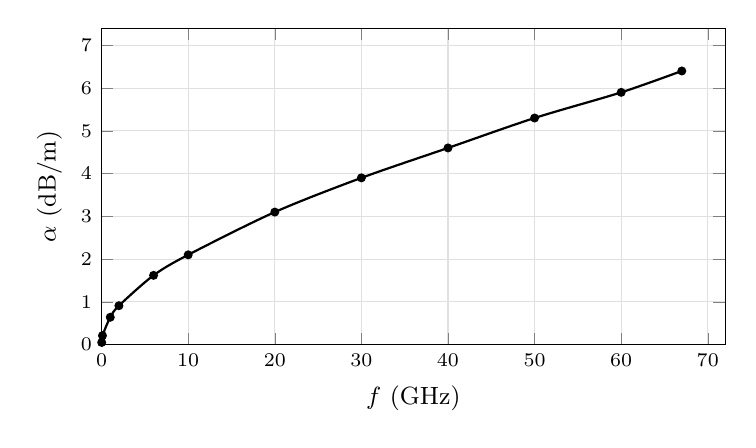
\begin{tikzpicture}
    \begin{axis}[width=9.5cm,height=5.6cm,
        xlabel={$f$ (GHz)},ylabel={$\alpha$ (dB/m)},
        xmin=0,xmax=72,ymin=0,ymax=7.4,
        xtick={0,10,20,30,40,50,60,70},ytick={0,1,2,3,4,5,6,7},
        grid=both,grid style={black!12},
        tick label style={font=\scriptsize},label style={font=\small}]
      \addplot[thick,mark=*,mark size=1.2pt,smooth] coordinates {
        (0.01,0.05) (0.1,0.21) (1,0.64) (2,0.91) (6,1.62) (10,2.1)
        (20,3.1) (30,3.9) (40,4.6) (50,5.3) (60,5.9) (67,6.4)};
    \end{axis}
  \end{tikzpicture}
  \caption*{\small Atténuation $\alpha$ des signaux RF dans un câble coaxial de
  longueur $1$ m, en fonction de la fréquence. $\alpha$ increases monotonically
  with frequency $\omega$.}
\end{figure}

\begin{figure}[h!]
  \centering
  \small
  \begin{tabular}{lccccccccc}
    \toprule
    $f$ & $10$ MHz & $0{,}1$ GHz & $1$ GHz & $2$ GHz & $6$ GHz & $10$ GHz & $20$ GHz & $40$ GHz & $67$ GHz \\
    \midrule
    $\alpha$ (dB/m) & $0{,}05$ & $0{,}21$ & $0{,}64$ & $0{,}91$ & $1{,}62$ & $2{,}1$ & $3{,}1$ & $4{,}6$ & $6{,}4$ \\
    $P_{\text{out}}$ (mW) & $0{,}99$ & $0{,}95$ & $0{,}86$ & $0{,}81$ & $0{,}69$ & $0{,}62$ & $0{,}49$ & $0{,}35$ & $0{,}23$ \\
    \bottomrule
  \end{tabular}
  \caption*{\small Output power of a $1$ m câble coaxial fed with
  $1$ mW $=0$ dBm.}
\end{figure}

\begin{example}[Reading the cable table]
  À $10$ MHz, $\alpha = 0{,}05$ dB/m, équivalent à $1\%$ d'atténuation de la
  puissance du signal, ce qui est négligeable. Par contre, à
  $1$ GHz (GSM à $890$\,--\,$960$ MHz), $\alpha = 0{,}64$ dB/m, soit environ
  $15\%$ d'atténuation, ce qui est loin d'être négligeable. À $6$ GHz (Wi-Fi à
  $5{,}2$\,--\,$5{,}7$ GHz), $\alpha = 1{,}62$ dB/m, soit environ $30\%$
  d'atténuation. Au-delà de $20$ GHz, $\alpha > 3$ dB/m, soit plus de $50\%$
  d'atténuation, et à $67$ GHz, $\alpha = 6{,}4$ dB/m, soit une puissance de
  signal atténuée de plus de $75\%$. Dans ce dernier cas, un signal ayant une
  puissance de $1$ mW à l'entrée du câble de $1$ m en ressort avec une
  puissance de $0{,}23$ mW.
\end{example}

\begin{conclusion}
  Attenuation of a signal RF is a serious issue in câble coaxial. For a
  signal BF it is not a concern at all. One metre of cable is a
  component, not a wire.
\end{conclusion}

\subsubsection{Affaiblissement en espace libre}
Si l'atténuation des signaux RF dans un câble peut être élevée, elle est
cependant bien inférieure à l'atténuation dans l'air.

\begin{definition}[Affaiblissement en espace libre]
  L'\textbf{affaiblissement en espace libre} (\textit{free-space path loss},
  FSPL) est la grandeur utilisée pour quantifier l'affaiblissement d'un signal
  RF dans l'air en fonction de la fréquence $f$ pour un signal se propageant
  entre une antenne d'émission (Tx) et une antenne de réception (Rx) séparées
  par une distance $d$ :
  \[\text{FSPL}=\left(\frac{4\pi d f}{c}\right)^{2},\qquad c=3\times 10^{8}\ \text{m/s}.\]
\end{definition}

The expression is stated here and used as a fact; its origin and derivation
come later with the bilan de liaison and the équation de Friis.
L'affaiblissement en espace libre FSPL augmente de manière
\textit{quadratique} en fonction de la fréquence $f$ et de la distance $d$
entre émetteur/récepteur. On exprime généralement cet affaiblissement en
échelle logarithmique :
\[\text{FSPL(dB)}=10\log_{10}\!\left(\frac{4\pi d f}{c}\right)^{2}
  =20\log_{10}(d)+20\log_{10}(f)-147{,}5,\]
with $d$ in metres and $f$ in hertz.

\begin{remark}
  The constant $-147{,}5$ is $20\log_{10}(4\pi/c)$ with $c$ in m/s; it is tied
  to those units. Feeding $d$ in km or $f$ in GHz changes the constant, so keep
  metres and hertz unless a formula explicitly says otherwise.
\end{remark}

\begin{figure}[h!]
  \centering
  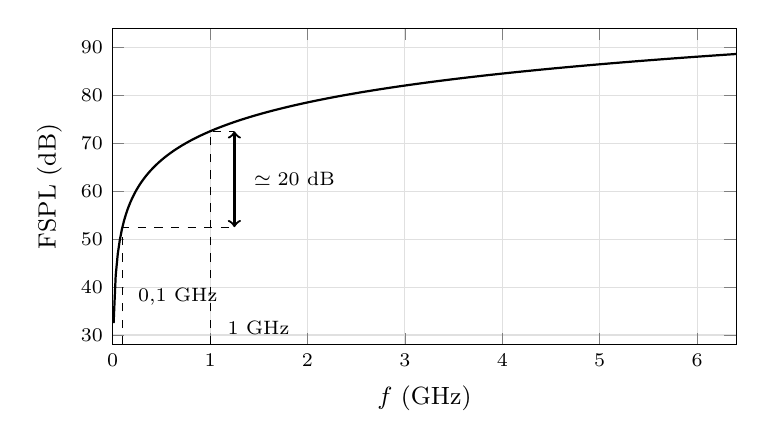
\begin{tikzpicture}
    \begin{axis}[width=9.5cm,height=5.6cm,
        xlabel={$f$ (GHz)},ylabel={FSPL (dB)},
        xmin=0,xmax=6.4,ymin=28,ymax=94,
        xtick={0,1,2,3,4,5,6},ytick={30,40,50,60,70,80,90},
        grid=both,grid style={black!12},
        tick label style={font=\scriptsize},label style={font=\small}]
      \addplot[thick,domain=0.01:6.4,samples=300]{72.5+20*log10(x)};
      \draw[dashed] (axis cs:0.1,28) -- (axis cs:0.1,52.5) -- (axis cs:1.25,52.5);
      \draw[dashed] (axis cs:1,28) -- (axis cs:1,72.5) -- (axis cs:1.25,72.5);
      \draw[<->,thick] (axis cs:1.25,52.5) -- (axis cs:1.25,72.5);
      \node[right,font=\scriptsize] at (axis cs:1.35,62.5) {$\simeq 20$ dB};
      \node[right,font=\scriptsize] at (axis cs:0.16,38) {$0{,}1$ GHz};
      \node[right,font=\scriptsize] at (axis cs:1.08,31.5) {$1$ GHz};
    \end{axis}
  \end{tikzpicture}
  \caption*{\small Atténuation en espace libre (FSPL) des signaux RF pour une
  distance émetteur/récepteur $d=100$ m.}
\end{figure}

\begin{example}[The $20$ dB that matters]
  Take $d = 100$ m. À $100$ MHz, le FSPL $=52{,}5$ dB tandis qu'à $1$ GHz (GSM à
  $890$\,--\,$960$ MHz), FSPL $=72{,}5$ dB, soit $20$ dB d'écart, ce qui
  signifie qu'un signal RF à la fréquence de $1$ GHz est $100$ fois plus
  atténué qu'un signal de $100$ MHz. Equivalently: a GSM $900$ MHz signal is
  attenuated $100$ times more than an FM radio signal at $88$\,--\,$108$ MHz
  over the same distance. L'affaiblissement des signaux devient beaucoup plus
  problématique aux fréquences RF qu'aux fréquences BF.
\end{example}

\begin{conclusion}
  Du fait de la très forte atténuation des signaux RF dans l'air, il est
  indispensable de les amplifier au niveau de l'émetteur d'une part
  (amplification de puissance, avant l'antenne Tx), et au niveau du récepteur
  d'autre part (amplification faible bruit, après l'antenne Rx).
  That is exactly why the PA and the LNA sit where they do in the functional
  diagram above, and why dispositifs d'adaptation d'impédance sit at every
  interface between them.
\end{conclusion}

\begin{remark}
  Tous les systèmes de télécommunications modernes possèdent des circuits
  électroniques qui remplissent les fonctions indiquées sur le schéma
  fonctionnel ci-dessus (modulation/démodulation numérique, conversion
  analogique/numérique \& numérique/analogique, mélange, oscillation,
  amplification de puissance/faible bruit, filtrage, rayonnement). Ces
  circuits sont complexes et la compréhension de leur fonctionnement
  nécessite des connaissances dans différents domaines (traitement du signal
  \& communications numériques, électronique numérique et analogique,
  électronique RF, antennes \& propagation RF). Celles-ci sont en pratique
  étudiées dans différentes UEs de 1ère année (ECE\_3TC21\_TP, APM\_3TC15\_TP,
  ECE\_3TC22\_TP) et surtout de 2ème année (filière TELECOM). This module owns
  the last two: RF electronics at the level of lignes de transmission and
  adaptation d'impédance, and antennes and propagation.
\end{remark}
